\documentclass{beamer}
\usepackage{qrcode}
%\usepackage{sansmathfonts}
\usepackage[T1]{fontenc}
\usepackage{mlmodern}
\usepackage{helvet}
\usepackage{DejaVuSansMono}
\usepackage{amsthm}
\usepackage{amssymb}
\usepackage{microtype}
\usepackage{color}

\newcommand{\Spec}{\mathrm{Spec}}


\newtheorem{defn}{{\bfseries Defn}}[section]
\newtheorem{thm}[defn]{{\bfseries Thm}}
\newtheorem{lem}[defn]{{\bfseries Lem}}
\newtheorem{prop}[defn]{Prop}
\newtheorem{ex}[defn]{{\bfseries Ex}}
\newtheorem{rem}[defn]{Rem}
\newtheorem{ques}[defn]{Qstn}

\newcommand{\lBrack}{[\![}
\newcommand{\rBrack}{]\!]}


\newcommand{\lParen}{(\!(}
\newcommand{\rParen}{)\!)}



%\renewcommand{\rmdefault}{\sfdefault}

\usepackage[english]{babel}

\usepackage[math]{blindtext}
\usepackage{tikz}
\usetikzlibrary{arrows.meta}
\usetikzlibrary{positioning}
\usetikzlibrary{graphs,graphdrawing} 
\usegdlibrary{trees}
\usegdlibrary{force}
\usegdlibrary{routing} 
\usegdlibrary{circular}
\usetikzlibrary{bending}
\usepackage{graphicx}

\usepackage{tikz-cd}









% Choose how your presentation looks.
%
% For more themes, color themes and font themes, see:
% 
%
\mode<presentation>
{
  \usetheme{default}      % or try Darmstadt, Madrid, Warsaw, ...
  \usecolortheme{default} % or try albatross, beaver, crane, ...
  \usefonttheme{default}  % or try serif, structurebold, ...
  \setbeamertemplate{navigation symbols}{}
  \setbeamertemplate{caption}[numbered]
} 

\title{Deformation quantisation and Airy structures}
\author{Michael Swaddle}
\institute{University of Melbourne}
\date{\today}


\definecolor{mBackground}{RGB}{252,252,248}
\definecolor{mNormal}{RGB}{36, 33, 36}
\definecolor{mTitle}{RGB}{52,48,52}
\definecolor{pink}{RGB}{255, 132, 255}
\newcommand{\changeurlcolor}[1]{\hypersetup{urlcolor=#1}}       

\setbeamercolor{background canvas}{bg=mBackground}
\setbeamercolor{normal text}{fg=mNormal}
\setbeamercolor{title}{fg=mTitle}
\setbeamercolor{frametitle}{fg=mTitle}
\setbeamercolor{block title}{fg=mTitle}



\newcommand\sbullet[1][.5]{\mathbin{\vcenter{\hbox{\scalebox{#1}{$\bullet$}}}}}
\newcommand{\sbt}{\sbullet[0.54]}


\setbeamertemplate{itemize items}[circle]
\setbeamertemplate{itemize item}{\color{pink}{$\sbt$}}



\usepackage{scalerel,stackengine}
\stackMath
\newcommand\reallywidehat[1]{%
\savestack{\tmpbox}{\stretchto{%
  \scaleto{%
    \scalerel*[\widthof{\ensuremath{#1}}]{\kern-.6pt\bigwedge\kern-.6pt}%
    {\rule[-\textheight/2]{1ex}{\textheight}}%WIDTH-LIMITED BIG WEDGE
  }{\textheight}% 
}{0.5ex}}%
\stackon[1pt]{#1}{\tmpbox}%
}
\parskip 1ex
\newcommand{\trightarrow}{\(\rightarrow\)}

%\newcommand{\Res}[1]{\underset{#1}{\operatorname{Res}}}
\DeclareMathOperator*{\Res}{Res} 




\hypersetup{
    colorlinks=true,
    breaklinks,
    linkcolor=pink,
    citecolor=pink,
    urlcolor=pink,
    filecolor=pink
}




\newcommand{\setsecbg}{
    \setbeamertemplate{background}{
    \begin{tikzpicture}
    \useasboundingbox  (0,0) rectangle(\the\paperwidth, \the\paperheight);
    \fill[color=mTitle] (0,0) rectangle(\the\paperwidth, \the\paperheight) ;   
    \end{tikzpicture}
    }
}    

\newcommand{\setslidebg}{
    \setbeamertemplate{background}{
    \begin{tikzpicture}
    \useasboundingbox  (0,0) rectangle(\the\paperwidth, \the\paperheight);
    \fill[color=mBackground] (0,0) rectangle(\the\paperwidth, \the\paperheight);   
    \end{tikzpicture}
    }
}    

\newcommand{\sectionframe}{
    \setsecbg
    \frame{\Large  \sectionpage}
    \setslidebg
}

\usepackage{caption}
\captionsetup[figure]{labelfont={color=mTitle}}

\DeclareMathOperator*{\colim}{colim}


\begin{document}





    \begin{frame}
        \titlepage
    \end{frame}
    

    \section{Warm up}
        
        

        \begin{frame}{Starting point}
        \begin{figure}[b]
        \begin{minipage}{0.12\textwidth} 
        \changeurlcolor{mNormal} \qrcode[height=1.2cm]{https://arxiv.org/abs/1701.09137}   
        \end{minipage} 
        \hfill 
        \begin{minipage}{0.85\textwidth} 
        \raggedright
        \emph{Airy structures and symplectic geometry of  topological recursion}, M. Kontsevich and  Y. Soibelman, 2017, {\color{pink}{\tt arXiv:1701.09137}} [math.AG]
        \end{minipage}
        \end{figure} 
        \end{frame}
    
        %\begin{frame}{Possible things to take away}
        %Hopefully, some knowledge of deformation quantisation.
        
        %The definition of an Airy structure.
        %\end{frame}
    
    
        \begin{frame}{Deformations}
        A formal deformation replaces a \( \mathbf{k} \)-algebra \((A,\cdot)\), with a non commutative \(\mathbf{k} \lBrack \hslash \rBrack \)-algebra \( (A_{\hslash},\star)\), such that
        \[ 0 \rightarrow \hslash A_{\hslash} \rightarrow A_{\hslash} \rightarrow A \rightarrow 0, \]
        eg \( A_{\hslash}/\hslash A_{\hslash} = A\).
        
        Gives a deformed product: \( a_{\hslash} \star b_{\hslash} = a \cdot b + O(\hslash)\).
        
        \emph{Deformation quantisation} is formal deformation with extra constraint. \(A\) is Poisson algebra, Poisson bracket \( \{ \cdot, \cdot\}\): 
        \[ a \star b - b \star a = \hslash \{ a, b\} + O(\hslash^2)\] 
        matches Poisson structure.
        
        \end{frame}    
            
        \begin{frame}
        \begin{ex}[Weyl algebra]
        Replacing the ring of functions \( \mathbf{k}[x,y]\), (with Poisson bracket \(\{ x,y\}=1)\), with a ring of operators \( \mathbf{k}[x,\hslash \frac{\partial}{\partial x} ]\lBrack \hslash \rBrack \) is a (representation of a) deformation quantisation.
        \end{ex} 
        
        Need a space on which these operators act -- wavefunctions.

        \end{frame}
        
        
        \begin{frame}{The big picture}
        Symplectic affine symplectic space \((W_\Sigma, \mathcal{O}(W_\Sigma))\).

        \begin{center}
        \begin{tikzpicture}[
            node distance=2cm and 3cm,
            ar/.style={->,>=latex},
            mynode/.style={
              draw,
              text width=3cm,
              minimum height=1cm,
              text centered
              }
            ]
            
            \node[mynode] (ar) {Airy structure\\ on \(\mathcal{O}(W_\Sigma\))};

            
            \node[mynode, right=of ar] (ls) {Lagrangian subvariety \( \mathcal{O}(\mathbb{L})\) };

            \node[mynode,below=of ar] (Asig) {A tensor \(A_\Sigma \cong \omega_{0,3}\)};

            
            \node[mynode,below=of ls] (tr) {Topological recursion \( \omega_{g,n}\)};

            \draw[ar] 
              (ls) -- node[right] {\parbox{3cm}{Deformation Quantisation}} (tr);
            \draw[ar] 
              (ar) -- node[above] {Encodes} (ls);
            \draw[ar] 
              (ar) -- node[above] {} (Asig);
            \draw[ar] 
              (Asig) -- node[above] {Initial data for} (tr);

        \end{tikzpicture}
        \[ 0 \rightarrow \mathcal{J} \rightarrow  \mathcal{O}(W_\Sigma) \rightarrow \mathcal{O}(\mathbb{L}) \rightarrow 0 \]
        \end{center}
        
        \( \omega_{g,n} \) meromorphic poly-differential.
        
    
        % linear symplectic vector space 
        % lagrangian subspaces
        % non degenerate (2,0) form \(\omega\)
        % quadratic 
        
        
        % coefficients of variety - tensors
        % coefficients turns out to be tensors
        % remind that describing geometry of subvariety
        % pictures are encoding lagrangian
        
        %lagrangian subvariety - tensors
        
        
        % history - quadratic lagrangian - quantisation understood - arise in givental, varieties
        
        % get lie algebra -> can quantise lie algebra
        % hamiltonians symplectic group
    \end{frame}
    
    \begin{frame}{What we added}
         Need \emph{deformation quantisation}, \( \mathcal{O}(W_\Sigma) \lBrack \hslash \rBrack \).
    
        This gives an understanding  of \emph{reduction} of {wavefunctions}, \( \psi_{\mathbb{L}}  \rightarrow \psi_{\mathcal{B}}\).
        
        \[ \psi_{\mathbb{L}} \in \text{Hom}\left( \widehat{\mathcal{O}}(W_\Sigma)\lBrack \hslash \rBrack / ( \mathcal{J} ) , \widehat{\mathcal{O}}(W_\Sigma)\lBrack \hslash \rBrack \right), \]
        
        Connection between \(A_\Sigma\) and the  \emph{Donagi Markman cubic}, which is a cohomology class: \([A_\Sigma]\)
    \[ a_{ijk} x^i x^j x^k  = S_{0,3} \cong A_\Sigma =  a_{ijk} x^i \otimes x^j \otimes x^k, \]

    \end{frame}

    \begin{frame} 
    \( \psi_{\mathbb{L}}\) produced by deformation quantisation. Wavefunctions are a generating function:
    \[ \psi_{\mathbb{L}} = \exp \left[ \frac{1}{\hslash} ( S_{0,3} +S_{0,4} + \dots ) + (  S_{1,1} + \dots ) + \hslash (  S_{2,1} + \dots ) \right], \]
    where \( S_{g,n} \cong \omega_{g,n}\). 
    
    \( \psi_{\mathcal{B}}\) depends on cohomology classes, 
    \[ \psi_{\mathcal{B}} = \exp \left[ \frac{1}{\hslash}\, \mathcal{S} \right] \]
    \( \mathcal{S}\) series in \(\hslash\) on \( \mathcal{B}\), \(\mathcal{B}\) moduli space of deformations of \(\Sigma\) in a surface.
    
    Quantisation of moduli space of deformations of curves?
    \end{frame}


    \begin{frame}{What else we added}
    
    Verified a formula for the reduction of wavefunctions following Kontsevich and Soibelman
    \begin{thm}
    \[ \psi_{\mathcal{B}} = \int D x\, \psi_{\mathbb{L}} \, \exp\left( \frac{1}{\hslash} Q(x^{\sbt}, z^{\sbt}) \right) \]
    \end{thm}
    \(Q\) determined from a fibre product. \(G \subset W_\Sigma\) coisotropic.
    \begin{center}
        \begin{tikzcd}[ampersand replacement=\&]
        \mathcal{O}_{W_\Sigma } \otimes_\mathbf{k}\mathcal{O}_{G }^{G^{\perp}}  \arrow[r] \arrow[d] \& \mathcal{O}_{G} \arrow[d]\\
        \mathcal{O}_{\mathbb{L}} \arrow[r] \&  \mathcal{O}_{G \cap {\mathbb{L}}}   \cong \mathcal{O}_{\mathcal{B}}
        \end{tikzcd}
    \end{center}
    \( \psi_{\mathcal{B}}\) associated to deformation quantisation of \( \mathcal{O}_{\mathcal{B}}\).
    \end{frame}
    
    
    \begin{frame}{Papers}
    \begin{figure}[t]
        \begin{minipage}{0.12\textwidth}    
        \changeurlcolor{mNormal}\qrcode[height=1.2cm]{https://arxiv.org/abs/2206.04848}
        \end{minipage} 
        \hfill
        \begin{minipage}{0.85\textwidth} 
        \raggedright
        \emph{Deformation quantisation of the conic and symplectic reduction of wavefunctions}, 
        M. Swaddle, 2022, {\color{pink}{\tt arXiv:2206.04848}} [math-ph] 
        \end{minipage}
    \end{figure}
    
    \begin{figure}[b]
        \begin{minipage}{0.12\textwidth}    
        \changeurlcolor{mNormal}\qrcode[height=1.2cm]{https://arxiv.org/abs/2012.00254} 
        \end{minipage} 
        \hfill 
        \begin{minipage}{0.85\textwidth}
        \raggedright
        \emph{Airy structures and deformations of curves in surfaces}, W. Chaimanowong, P. Norbury, M. Swaddle, and M. Tavakol, 2020, {\color{pink}{\tt 	arXiv:2012.00254}} [math.AG]
        \end{minipage}
        \end{figure}
    \end{frame}

    
    \begin{frame}{Outline}
    \tableofcontents
    \end{frame}

    \frame{\sectionpage}

    \begin{frame}{Formal completion of a ring}
    Complete at a maximal ideal \( \langle x \rangle \):
    \begin{ex} \[ \mathbf{k} \lBrack x \rBrack   = \lim_{n}  \frac{\mathbf{k}[x]}{\langle x \rangle^n} \]
    \end{ex}
    Limit is limit in category of rings, \( \mathbf{k}\lBrack x \rBrack \) is something all \( \mathbf{k}[x] / \langle x \rangle^n\) map into.
    
    More generally a terminal object \(R_I = \lim_n R/I^n\). 
    
    Actually think lazy evaluation, always think in terms of finite \(n\)-th quotient \(R/I^n\), and can always go to to \(n+1\) if needed.
    
    \begin{defn}\( \Spec( R/I^n)\) called the \(n\)-th formal neighbourhood.
    \end{defn} 
    \end{frame}
    
    \begin{frame}{Why is this important?}
    In the application to topological recursion, \( \mathbb{L}\) is only topologically a point in an infinite dimensional symplectic space \(W_\Sigma\). However, the formal neighbourhoods of \( \mathbb{L}\) contain rich information.
    \end{frame}
    
    
    
    % say more completion
    
    % defn of completion
    
    % why need completions
    % forced to do power series
    
    % L topologically a point in W 
    % look in formal neighbourhoods of point
    % model example something infinite dimensions, 
    % in that case underlying thing topologically a point
    % look in formal neighbourhoods
    % extract interesting information (tr etc)
    
    
    % example Lagrangian
    % symplectic affine spaces
    
    % add lagrangian closed poisson bracket
    
    % more definitions
    
    \begin{frame}{The conic}
    An important example to take away.
    
     \( \mathbf{k}\) field characteristic zero.
    
    \vspace{1em}
    \begin{ex}[Conic in the plane]
    Consider \( \mathbf{k}[x,y]\) as Poisson algebra, Poisson bracket \( \{y,x\}=1\).
    
    Example Lagrangian:
    \[\mathbb{L} = \Spec \left( \frac{\mathbf{k}[x,y]} {  \mathcal{J}(\mathbb{L})} \right) \]
    where 
    \(  \mathcal{J}(\mathbb{L}) = \langle -y +  x^2 + 2 \,x\, y + y^2\rangle\)
    \end{ex} 
    Ideal must be closed under Poisson bracket: 
    \[ \{ \mathcal{J}, \mathcal{J} \}  \subseteq \mathcal{J} \]
    \end{frame} 
    %wait I guess I mean R/I , R/I = 
    
    % limit first, then completion
    

    
    
    \begin{frame} 
    \begin{figure}
    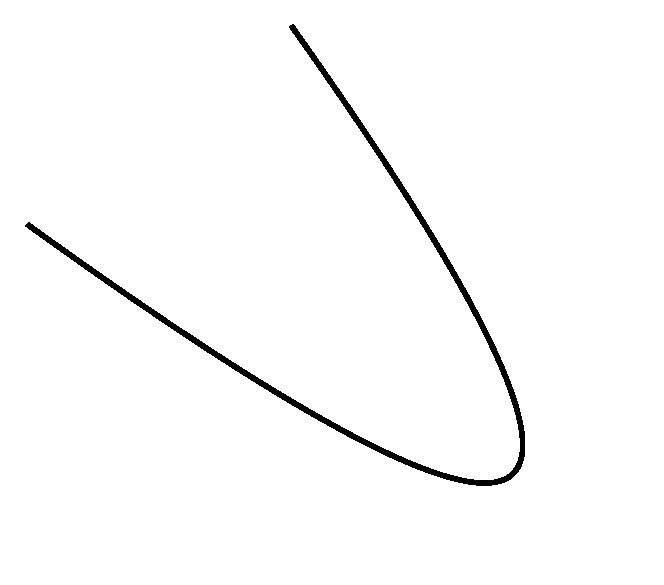
\includegraphics[width=4cm]{sections/out.pdf}
    \caption{\(-y+x^2+2 xy+y^2=0\)}
    \end{figure}    
    \end{frame} 
    
    \begin{frame}
    Solve \(-y + x^2 + 2\, x\, y + y^2 = 0\) for \(y(x)=u_0(x)\) via fixed point iteration. 
    
    Algebraically: completion at maximal ideal \( \langle x, y \rangle \):
    \[ \widehat{\mathbb{L}} = \mathrm{Spf} \left( \mathbf{k}[\![x,y ]\!]/ \langle y - u_0 \rangle \right) \]
    Formal series
    \[ u_0 = x^2 + 2 x^3 + 5 x^4 + \dots \]
    Encodes the \emph{Catalan numbers}:
    \[ \{1,2,5,14,\dots \}\]
    Formal series can contain interesting data. 
    \end{frame}
    
    \begin{frame}{Fixed point iteration}
        Finding the formal series.
        
        Initial condition \(y^{[0]} = 0\).
        \begin{align*} 
        y^{[n]} &= x^2 + 2 \,x\, y^{[n-1]} + y^{[n-1]}\, y^{[n-1]} \\
        y^{[1]} &= x^2 \\
        y^{[2]} &= x^2 + 2 \, x^3 + (x^2)\, (x^2) 
        \end{align*}
        Coefficients stabilise and \(y^{[n]} \rightarrow u_0(x)\). This idea generalises to the infinite dimensional case.
    \end{frame}
    
    
    \begin{frame}{Trees}
    Catalan numbers count rooted binary trees (notion of left/right)
    \begin{center}
    \begin{tabular}{c c c } 
    
    \tikz [tree layout, baseline=(x0.base), grow'=up, significant sep=1em, sibling distance=7mm, level distance=7mm]
     \graph {
        [nodes={circle, draw, inner sep=0pt, minimum size=2mm, as =}]{ x0};
        // [nodes={circle, inner sep=0pt, minimum size=2mm, fill, as=}]{ x0 -- x1 };
        // [nodes={circle, fill={pink} }]{ x1 -- {x2,x3}};
    };  
    
    &
    \tikz [ baseline=(a.base), tree layout, significant sep=1em, grow'=up, sibling distance=7mm, level distance=7mm]
    \graph {
        [nodes={circle, draw, inner sep=0pt, minimum size=2mm, as =}]{ a};
        // [nodes={circle, inner sep=0pt, minimum size=2mm, fill, as=}]{a -- {b--{c}} };
        // [nodes={circle, fill={pink} }]{b-- d};
        // [nodes={circle, fill={pink} }]{c --{e,f}};
        };
    & 
    
    \tikz [ baseline=(a.base), tree layout, significant sep=1em, grow'=up, sibling distance=7mm, level distance=7mm]
    \graph {
        [nodes={circle, draw, inner sep=0pt, minimum size=2mm, as =}]{ a };
        // [nodes={circle, inner sep=0pt, minimum size=2mm, fill, as=}]{ a -- { b-- {c,d}} };
        // [nodes={circle, fill={pink} }]{ c -- {e,f}};
        // [nodes={circle, fill={pink} }]{ d -- {g,h}};
        };
    
    \tikz [ baseline=(a.base), binary tree layout, significant sep=1em, grow'=up, sibling distance=7mm, level distance=7mm]
    \graph {
        [nodes={circle, draw, inner sep=0pt, minimum size=2mm, as =}]{ a };
        // [nodes={circle, inner sep=0pt, minimum size=2mm, fill, as=}]{ a -- b -- { d -- {e }} };
        // [nodes={circle, fill={pink} }]{ b -- c};
        // [nodes={circle, fill={pink} }]{ d -- f};
        // [nodes={circle, fill={pink} }]{ e -- {g,h}};
        };
    \\
    & &  \\ 
    \(x^2\) & \( 2 x^3\) &  \( 5 x^4 \)
    \end{tabular}
    \end{center}
    Drawn up to \( \cong\).
    \[ u_0(x) = x^2 + 2 x^3 + 5 x^4 + \dots \]
    \end{frame}
    
    
    \begin{frame}{Preview: Airy structures}
    Going to be a weighting with coefficients \( ( a , b , c )\)
    \[ \mathbf{k}[x,y] / \langle-y + {\color{pink} a}\, x^2 + 2 \,  {\color{pink} b} \,x\, y +  {\color{pink} c}\, y^2\rangle \]
    This will put a label/weighting on nodes in the tree.
    \[ u_0 = ({\color{pink} a})\, x^2 + ({\color{pink} 2\, b\, a} )\,x^2 + ({\color{pink} 4 \, b^2\, a + c \, a^2 } ) x^4 + \dots \]
    \end{frame}
    
    
    
    \begin{frame}{Preview}
    We will generalise this example following Kontsevich and Soibelman to arbitrary (and infinite) dimensions.
    \[ x\rightarrow \{x^1,x^2, \dots \}, y \rightarrow \{y_1, y_2 \dots\}\] 
    Quadratic replaced by a collection of polynomials \(H_i\).
    \[ H_i = -y_i + a_{ijk}x^j x^k + 2 b_{ij}^k x^j y_k + c_{i}^{jk} y_{j} y_k\]
    Scalar coefficients become tensors \(a \rightarrow a_{ijk}\).

    Coefficients in series \(u_{0}(x) \rightarrow u_{0,i}(x^{\sbt})\) become contraction of tensors, eg: 
    \[u_{0,i} = a_{ijk} x^j x^k + 2 b_{ij}^k a_{k st}x^j x^s x^t + \dots \]
    
    
    
    \end{frame}

    \begin{frame}{Finiteness}
    A key component is the choice of topology.
    
    Need to ensure sums converge or there is finiteness.
    
    Need to ensure contraction of tensors is finite, eg:
    \[ 2 b_{ij}^k a_{k st}\]
    
    

    %Pair a finite list and an infinite list
    %\[ \texttt{sum} \quad \$ \quad  \texttt{zipWith} \quad (*) \quad [1,2,\dots,N] \quad [1,2,\dots]\]
    \end{frame}

    
    %  x2 --[bend right=20] x4 , 
    % x2--[bend left=20] x4 , 
    
    
    % \quad 
 

    \section{Topological recursion}
    
    
        \frame{\sectionpage}

 
 \begin{frame}{Topological recursion}
    \( \Sigma \) curve  inside \(\mathbb{C}^2\), with divisor \( R \). % one dimensional scheme
    
    Algorithm -- recursion in two non-negative integers \(g,n\). 

    Produces a collection of \emph{meromorphic}, \emph{symmetric} polydifferentials or invariants \(  \omega_{g,n}\) 
    \[ \omega_{g,n} \in \Gamma(  \left(\Sigma - R \right)^n, \kappa_\Sigma^{\boxtimes n} )   .\] 
    \begin{ex}
    \[ \omega_{0,1} = 2 z_1^2 dz_1 ,\quad  \omega_{0,2} = \frac{dz_1 \, dz_2}{(z_1^2 - z_2^2) }. \]
    \end{ex}
    
    Why do we care? \( \omega_{g,n}\) compute interesting numbers, string theory, enumerative geometry etc.
    \end{frame} 
    
    
    
    \begin{frame} 
    Initial conditions \( \omega_{0,3}\), \(\omega_{1,1}\) given.
    \begin{defn}[Topological recursion]
    \begin{align*}\omega_{g,n}(z_{\sbt}) =& \sum_{\alpha \in \text{Ram} } \Res_{z = \alpha}  K(z_1, z) \Big[ \omega_{g-1, n+1} (z, \sigma_\alpha(z), z_2, \dots, z_n) \\
    + &\sum_{\substack{g_1 + g_2 = g \\ I_1 \sqcup I_2 = \{z_2\dots,z_n\} }} \omega_{g_1, \# I_1+1}(z,I_1) \, \omega_{g_2, \#I_2  +1}(\sigma(z), I_2) \Big]
    \end{align*}
    \( \sigma \) local involution at ramification point, \( K(z_1,z)\) recursion kernel, \( z_{\sbt} = (z_1, \dots z_n)\).
    \end{defn} 
    Take away: Quadratic relations in \( \omega_{g,n}\). Could it look like relations from a conic?
    \end{frame}
    
    \begin{frame}
        \begin{center}
        

\tikzset{every picture/.style={line width=0.75pt}} %set default line width to 0.75pt        

\begin{tikzpicture}[x=0.75pt,y=0.75pt,yscale=0.8,xscale=0.8]
%uncomment if require: \path (0,475); %set diagram left start at 0, and has height of 475

%Shape: Ellipse [id:dp47766951388601575] 
\draw   (117.44,140) .. controls (117.44,134.48) and (119.68,130) .. (122.44,130) .. controls (125.2,130) and (127.44,134.48) .. (127.44,140) .. controls (127.44,145.52) and (125.2,150) .. (122.44,150) .. controls (119.68,150) and (117.44,145.52) .. (117.44,140) -- cycle ;
%Shape: Ellipse [id:dp2213117305497102] 
\draw   (117.44,178.8) .. controls (117.44,173.28) and (119.68,168.8) .. (122.44,168.8) .. controls (125.2,168.8) and (127.44,173.28) .. (127.44,178.8) .. controls (127.44,184.33) and (125.2,188.8) .. (122.44,188.8) .. controls (119.68,188.8) and (117.44,184.33) .. (117.44,178.8) -- cycle ;
%Curve Lines [id:da6254818543814082] 
\draw    (82.44,150) .. controls (99.71,153.2) and (100.28,127) .. (122.44,130) ;


%Curve Lines [id:da26678157319223816] 
\draw    (82.44,170) .. controls (92.38,169.2) and (95.36,171.58) .. (100.46,177.57) .. controls (105.55,183.56) and (111.09,190.25) .. (122.44,188.8) ;


%Shape: Ellipse [id:dp13037643339418226] 
\draw   (352.56,141) .. controls (352.56,135.48) and (354.8,131) .. (357.56,131) .. controls (360.32,131) and (362.56,135.48) .. (362.56,141) .. controls (362.56,146.52) and (360.32,151) .. (357.56,151) .. controls (354.8,151) and (352.56,146.52) .. (352.56,141) -- cycle ;
%Shape: Ellipse [id:dp17263407292053756] 
\draw   (352.56,179.8) .. controls (352.56,174.28) and (354.8,169.8) .. (357.56,169.8) .. controls (360.32,169.8) and (362.56,174.28) .. (362.56,179.8) .. controls (362.56,185.32) and (360.32,189.8) .. (357.56,189.8) .. controls (354.8,189.8) and (352.56,185.32) .. (352.56,179.8) -- cycle ;
%Curve Lines [id:da07654552783686674] 
\draw    (317.56,151) .. controls (336.82,151.2) and (335.39,128) .. (357.56,131) ;


%Curve Lines [id:da9658431109856747] 
\draw    (317.56,171) .. controls (326.82,171.2) and (330.48,172.58) .. (335.58,178.57) .. controls (340.67,184.56) and (346.21,191.24) .. (357.56,189.8) ;


%Curve Lines [id:da5347071930943992] 
\draw    (357.56,151) .. controls (343.39,151) and (342.39,171) .. (357.56,169.8) ;


%Shape: Ellipse [id:dp3047856800313534] 
\draw   (432.56,100) .. controls (432.56,94.48) and (434.8,90) .. (437.56,90) .. controls (440.32,90) and (442.56,94.48) .. (442.56,100) .. controls (442.56,105.52) and (440.32,110) .. (437.56,110) .. controls (434.8,110) and (432.56,105.52) .. (432.56,100) -- cycle ;
%Shape: Ellipse [id:dp604261263939661] 
\draw   (432.56,150) .. controls (432.56,144.48) and (434.8,140) .. (437.56,140) .. controls (440.32,140) and (442.56,144.48) .. (442.56,150) .. controls (442.56,155.52) and (440.32,160) .. (437.56,160) .. controls (434.8,160) and (432.56,155.52) .. (432.56,150) -- cycle ;
%Shape: Ellipse [id:dp011621115124847092] 
\draw   (422.56,210) .. controls (422.56,204.48) and (424.8,200) .. (427.56,200) .. controls (430.32,200) and (432.56,204.48) .. (432.56,210) .. controls (432.56,215.52) and (430.32,220) .. (427.56,220) .. controls (424.8,220) and (422.56,215.52) .. (422.56,210) -- cycle ;
%Curve Lines [id:da570536589787372] 
\draw    (377.56,130) .. controls (391.91,120.93) and (390.54,101.73) .. (402.56,100) .. controls (414.58,98.27) and (427.91,90.93) .. (437.56,90) ;


%Curve Lines [id:da47026968306688344] 
\draw    (377.56,150) .. controls (409.39,149) and (415.91,160.93) .. (437.56,160) ;


%Curve Lines [id:da10402241670297141] 
\draw    (437.56,110) .. controls (423.39,117) and (430.39,137) .. (437.56,140) ;


%Curve Lines [id:da7257812222165501] 
\draw    (404.48,137.77) .. controls (409.31,132.3) and (419.91,134.09) .. (422.9,140.41) ;


%Curve Lines [id:da1333862640100011] 
\draw    (403.69,136.32) .. controls (406.73,143.82) and (421.01,145.03) .. (423.95,138.9) ;



%Curve Lines [id:da9669557373363992] 
\draw    (401.88,118.32) .. controls (402.34,111.04) and (411.8,105.95) .. (418.05,109.11) ;


%Curve Lines [id:da3422827424389957] 
\draw    (400.37,117.67) .. controls (407.38,121.72) and (419.39,113.9) .. (417.94,107.27) ;



%Curve Lines [id:da9799334827307091] 
\draw    (377.56,190) .. controls (394.16,195.2) and (384.41,201.13) .. (396.16,206.53) .. controls (407.91,211.93) and (414.91,219.93) .. (427.56,220) ;


%Curve Lines [id:da9139019865430383] 
\draw    (396.15,187.78) .. controls (403.28,186.28) and (410.73,194.03) .. (409.35,200.89) ;


%Curve Lines [id:da4926725298466649] 
\draw    (396.37,186.16) .. controls (394.34,193.99) and (405.09,203.47) .. (411.1,200.3) ;



%Curve Lines [id:da8231578381022252] 
\draw    (377.56,170) .. controls (396.82,173.2) and (406.16,178.53) .. (410.82,183.87) .. controls (415.49,189.2) and (415.49,195.87) .. (427.56,200) ;


%Curve Lines [id:da41952521800040865] 
\draw    (317.56,151) .. controls (308.16,152.53) and (306.82,169.87) .. (317.56,171) ;


%Curve Lines [id:da022423481574913584] 
\draw    (377.56,130) .. controls (368.16,131.53) and (366.82,148.87) .. (377.56,150) ;


%Curve Lines [id:da9251927665164891] 
\draw    (377.56,170) .. controls (368.16,171.53) and (366.82,188.87) .. (377.56,190) ;


%Curve Lines [id:da23000894520127613] 
\draw    (317.56,171) .. controls (326.82,171.2) and (330.48,172.58) .. (335.58,178.57) .. controls (340.67,184.56) and (346.21,191.24) .. (357.56,189.8) ;


%Curve Lines [id:da10195049737374684] 
\draw    (122.44,150) .. controls (108.28,150) and (107.28,170) .. (122.44,168.8) ;


%Curve Lines [id:da5107062925199526] 
\draw    (142.44,150) .. controls (156.28,150) and (156.28,170) .. (142.44,170) ;


%Shape: Ellipse [id:dp3889460224785426] 
\draw   (207.44,120) .. controls (207.44,114.48) and (209.68,110) .. (212.44,110) .. controls (215.2,110) and (217.44,114.48) .. (217.44,120) .. controls (217.44,125.52) and (215.2,130) .. (212.44,130) .. controls (209.68,130) and (207.44,125.52) .. (207.44,120) -- cycle ;
%Shape: Ellipse [id:dp9770499883484128] 
\draw   (207.44,160) .. controls (207.44,154.48) and (209.68,150) .. (212.44,150) .. controls (215.2,150) and (217.44,154.48) .. (217.44,160) .. controls (217.44,165.52) and (215.2,170) .. (212.44,170) .. controls (209.68,170) and (207.44,165.52) .. (207.44,160) -- cycle ;
%Shape: Ellipse [id:dp4597094401087267] 
\draw   (207.44,200) .. controls (207.44,194.48) and (209.68,190) .. (212.44,190) .. controls (215.2,190) and (217.44,194.48) .. (217.44,200) .. controls (217.44,205.52) and (215.2,210) .. (212.44,210) .. controls (209.68,210) and (207.44,205.52) .. (207.44,200) -- cycle ;
%Shape: Boxed Bezier Curve [id:dp4201913915112617] 
\draw    (142.44,130) .. controls (168.28,132) and (174.28,118) .. (212.44,110) ;


%Curve Lines [id:da17496795078002492] 
\draw    (212.44,130) .. controls (198.28,130) and (197.28,151.2) .. (212.44,150) ;


%Straight Lines [id:da8933167588243608] 
\draw  [dash pattern={on 4.5pt off 4.5pt}]  (177.44,160) ;


%Shape: Boxed Bezier Curve [id:dp20175324397284145] 
\draw    (142.44,190.38) .. controls (168.28,188.42) and (174.28,202.15) .. (212.44,210) ;


%Curve Lines [id:da7870873777983136] 
\draw    (212.44,170) .. controls (198.28,170) and (197.28,191.2) .. (212.44,190) ;


%Curve Lines [id:da8945713210334673] 
\draw    (317.56,171) .. controls (326.82,171.2) and (330.48,172.58) .. (335.58,178.57) .. controls (340.67,184.56) and (346.21,191.24) .. (357.56,189.8) ;


%Curve Lines [id:da6694044469732641] 
\draw    (168.22,146.07) .. controls (171.1,139.38) and (181.73,137.76) .. (186.54,142.84) ;


%Curve Lines [id:da5731533719506826] 
\draw    (167.01,144.95) .. controls (172.25,151.12) and (186.19,147.81) .. (187.06,141.07) ;



%Curve Lines [id:da02679938946556648] 
\draw    (168.62,174.02) .. controls (174.06,169.17) and (184.37,172.19) .. (186.6,178.82) ;


%Curve Lines [id:da8638414158098124] 
\draw    (168,172.5) .. controls (170.14,180.3) and (184.19,183.18) .. (187.82,177.44) ;



%Curve Lines [id:da5955732991885125] 
\draw    (142.44,130) .. controls (133.04,131.53) and (131.71,148.87) .. (142.44,150) ;


%Curve Lines [id:da21844641699333922] 
\draw    (142.44,170.38) .. controls (133.04,171.92) and (131.71,189.25) .. (142.44,190.38) ;


%Curve Lines [id:da22082602480849645] 
\draw    (82.44,150) .. controls (73.04,151.53) and (71.71,168.87) .. (82.44,170) ;



% Text Node
\draw (235.44,160) node   {$+$};
% Text Node
\draw (279,164.5) node   {\tiny $\underset{\substack{g_1 + g_2 = g \\ I_1 \sqcup I_2 }}{\displaystyle{\Sigma}}$ };
% Text Node
\draw (168,100) node   {\tiny $\omega _{g-1,n+1}$};
% Text Node
\draw (386.5,82) node   {\tiny $\omega _{g_{1} ,\#I_{1}}$};
% Text Node
\draw (87.5,190) node   {$K$};
% Text Node
\draw (386.5,222) node   {\tiny $\omega _{g_{2} ,\#I_{2}}$};


\end{tikzpicture}

        \end{center}
    \end{frame}
    
        
    \begin{frame}
    For \(g=0\), the diagrams look a bit like the binary trees.
    
    Binary tree a bit like a possible skeleton. 
    
    Thicken the trees out.
    \end{frame}    
        
    %\begin{frame}
    %Natural reason for the existence of the topological recursion relations?
    %\end{frame}    
    
        
    \begin{frame}{Vector space of differentials}
    Infinite dimensional vector space \(W\) of meromorphic differentials with zero residue, \( W \subset \mathrm{Vec}(\mathbf{k}\lParen z \rParen dz) \), 
    \vspace{1em}
    \begin{ex}
    \[ z\, dz, \quad \frac{dz}{z^2} \in W\]
    \end{ex}
    Want to use this vector space to build tensors -- the  \(\omega_{g,n} \in \text{Sym}(W)\)
    
    \(\omega_{g,n}\) exist because of natural geometry.
    
    This explained by doing algebraic geometry over \(W\), look at rings \( \text{Sym}(W) \cong \mathbf{k}[\mathcal{B}_W]\).
    \end{frame}
    
    \section{Topological vector spaces}
        
        
   \frame{\sectionpage}
 
    \begin{frame}
     Machinery to build tensors in infinite dimensions.
    \end{frame}
    
    \begin{frame}{Lagrangians and symplectic geometry}
        \begin{itemize}
        \item \(W\) symplectic vector space over \( \mathbf{k}\): Vector space with symplectic form \( \omega : W \times W \rightarrow \mathbf{k}\), (alternating, bilinear, nondegenerate). 
        \item Let \( U \subset W\). Define the \emph{symplectic complement}:
        \[ U^{\perp} = \{ v \in W | \omega(u,v) = 0 \; \forall \; u \in U \} \]
        \item \( L \subset W\) is \emph{Lagrangian} if \( L^{\perp} = L \).
        \item Polarisation \(W = V \oplus V^*\).
        \end{itemize}
    \end{frame}

    
    \begin{frame}{Discrete topology}
    
     \begin{defn}[Discrete topology]
        Let \(X\) be a set. The \emph{discrete topology} on \(X\) is given by defining every subset as open, (and equivalently closed).
    \end{defn}
    
    The discrete topology is the topology that best captures the set theoretic structure of a space. Individual points in the discrete topology define open sets.

    \end{frame}    


    \begin{frame}
    Apply this topology to an infinite dimensional vector space \(V\), over \( \mathbf{k}\) also with the discrete topology.
    
    All discrete topological vector spaces look like \( \mathbf{k}^{\omega}\), where \( \omega\) is some ordinal, 
    \[ \mathbf{k}^{\infty} = \colim_n \oplus_n \mathbf{k}\]
    \end{frame}
    
    \begin{frame}{Discrete topological vector spaces}
    
     \begin{lem}
        If \(V\) is a discrete topological \(\mathbf{k}\)-vector space, and \(\dim(V)>0\), then necessarily \( \mathbf{k}\) must have the discrete topology. 
        
        Alternatively if \(V = \{ 0\}\), then \(\mathbf{k}\) can have any topology. 
        \end{lem} 
    
    From the requirement that multiplication is continuous.
    \end{frame}

    \begin{frame}{Discrete topological vector spaces}
    
    \begin{lem}[Properties of the discrete topology] 
        Let \(V\) be a  discrete topological \( \mathbf{k}\)-vector space. 
        \begin{itemize}
            \item Convergent sequences of elements of \(V\) are eventually constant. 
            \item \(V\) is Hausdorff.
            \item If \( \dim(V) > 1\), then \(V\) is fully disconnected.
        \end{itemize}
        \end{lem}
    \end{frame}



    \begin{frame}{Why discrete topology?}
    To describe a space, we consider functions on a space. For a discrete topological space \(X\), and any other topological space \(Y\), all functions \(f : X \rightarrow Y\) are continuous. Further they are equivalent to maps between the underlying sets.
    
    Also imposes strong finiteness to vectors.
    
    Every vector can be represented by a sequence with only finitely many non zero coefficients:
    \[ (c_0, \dots , c_N, 0, 0, \dots)\]
    for some finite \(N\), or 
    \[ \sum^{N}_{i=0} c_i\, e_i \]
    \end{frame}
    
 

    \begin{frame}{Tate spaces}
        \begin{defn}[Tate space]
            A \emph{Tate space}, \(W\), is a topological vector space (or more generally topological module) of the form
            \(W= V \oplus U^*\), where \(V\) and \(U\) are topological vector spaces with the discrete topology.
        \end{defn}
    
    The topological dual \(U^{*} \subseteq \mathrm{Hom}(U,\mathbf{k})\) naturally has locally linearly compact topology.  
    \end{frame}
    
    \begin{frame}
        When \(U = V\), then \(W\) is a \emph{strong symplectic} topological vector space, which means \(W = W^{*}\)
        
        Strong symplectic structure is equivalent to a choice of polarisation, we can write out Darboux coordinates, exists bases. 

    \end{frame}

    
    \begin{frame}{Examples}
       The Tate space \(W_{\text{Airy}}= V_{\text{Airy}} \oplus L_{\text{Airy}} = V_{\text{Airy}} \oplus (V_{\text{Airy}})^* \).
        \begin{itemize}
            \item   \(V_{\text{Airy}} \cong \mathrm{Vec}( z^{-1} \mathbf{k}[z^{-1}]dz)\),
            \item \(L_{\text{Airy}} \cong  \mathrm{Vec}(\mathbf{k}[\![z]\!]dz)\). 
        \end{itemize}
        \(x^i \in V_{\text{Airy}}\) represents a meromorphic differential. 
        
        \(y_i \in L_{\text{Airy}}  \) represents a formal holomorphic differential (only positive powers of \(z^k\)).
        
        \(y_i\) are coordinates on \(V_{\text{Airy}}\) etc
        
    \end{frame}
    
    \begin{frame}{Finiteness}
    Can pair a Laurent polynomial with a formal series, looking at the \emph{residue}, which is the \(1/z\)-term, always finite.
    \[ \left(\frac{1}{z} + \frac{1}{z^2}\right) \left( 1 + z + z^2 + z^3 + \dots \right) = \frac{1}{z^2} + \frac{2}{z}+\dots\]
    \end{frame}
    
    
    \begin{frame}{Examples}
             \( \Sigma \) Riemann surface with divisor \(R\) 
            \begin{itemize}
                \item \(V_\Sigma\) = global meromorphic differentials on \(\Sigma\) with zero A periods. 
                \item \(L_\Sigma \) = holomorphic differentials.
            \end{itemize}
            \(V_\Sigma\), \(L_\Sigma\) built from \(|R|\) copies of \(V_{\text{Airy}}\), \(L_{\text{Airy}}\)
    \end{frame}
    
    \begin{frame}{Doing algebraic geometry over \(W\)}
        Let \(V\) be vector space with discrete topology. Let \(W = V \oplus V^*\).
        \begin{itemize}
            \item Canonical basis \(\mathcal{B}\), \(  x^i \in V\) and \( y_i \in V^*\).
            \item Algebraic geometry on \(W\), look at a ring \( \mathbf{k}[\mathcal{B}^*]\).
        \end{itemize}
        \emph{Note}: \(x^i\) are coordinates on \(V^*\), 
        \(y_i\) are coordinates on \(V\). 

    \end{frame}

    \begin{frame}{Algebraic analog}%%  move up to algebraic geometry over W
    Pro/ind-infinite rings:
    \begin{align*} 
    \mathbf{k}[\mathcal{B}_{L^*}] &= \colim_n \mathbf{k}[x^1, \dots x^n]\\
     \mathbf{k} [\mathcal{B}_{V^*} ] &= \lim_n \mathbf{k}[y_1, \dots y_n]
     \end{align*}
    Both have infinitely many variables. 
     
    Finite sums of \(x^{\sbt}\), bound in degree, basically polynomials:
    \[ (x^1)^2 + (x^2), \quad  (x^{10000}) + (x^{3})^4, \] 
    Infinite sums of \(y_{\sbt}\), but bound in degree:
    \[ (y_1 + y_1^2 + \dots +y_1^N) + (y_2  + y_2^2) + \dots + y_{\infty}\]
    \end{frame}
    
    \begin{frame}
    Do algebraic geometry over \(W\), so look at the ring:
    \[ \mathcal{O}(W) = \mathbf{k}[\mathcal{B}_{L^*}] \otimes_{\mathbf{k}} \mathbf{k} [\mathcal{B}_{V^*} ]\]
    Inside this look at some ideal generated by a collection \(H_i\): 
    \[  H_i = a_{ijk} x^j x^k + 2 b_{ij}^k x^j y_k + c_i^{jk} y_j y_k - y_i\] 
    Note in infinite dimensions \( a_{ijk}\) must only pair with finitely many \(x^i\).
    \end{frame}

    \begin{frame}{In infinite dimensions}
        Only finite sums of \(x^i\) allowed imposed in tensors.
    \end{frame}

    \begin{frame}{Poisson structure}
        \emph{Poisson bracket},  \( \{ ,  \} : \mathbf{k}[\mathcal{B}^*] \times \mathbf{k}[\mathcal{B}^*] \rightarrow \mathbf{k}[\mathcal{B}^*]\). 
        
        Defined on basis:
        \[ \{ x^i, y_j \} = \delta_j^i , \quad \{ x^i , x^j\} = 0, \quad \{ y_i, y_j\} = 0.\]
    \end{frame}
       
    \begin{frame}{Poisson structure}
        Symplectic from the Poisson structure:
        \begin{itemize}
            \item Poisson bracket defines a symplectic form \( \omega\). Let \( f \in \mathbf{k}[\mathcal{B}^*]\). Define vector field (derivation) \( X_f = \{ f, \cdot \}. \) Then \( \omega\) is chosen so
            \[ \{ f, g\} = \omega(X_f , X_g ) \]
        \end{itemize}
        Now \(W\) is a symplectic vector space, and \(V^* \cong L\) is Lagrangian.
    \end{frame}
    
    
    \begin{frame}{No essential singularities}
    Finiteness in the \(V_\Sigma\) is important. Need finite sums (no essential singularities).        
    \end{frame}
    
    

    
    \section{Deformation quantisation}
        \frame{\sectionpage}

\begin{frame}
How do we get the particular tensors \(\omega_{g,n}\).

Answer: Deformation quantisation.
\end{frame}


\begin{frame}{Formal deformations}
Let \( (X,\mathcal{O}_X)\) be a scheme over \( \mathbf{k}\).
\vspace{1em}
\begin{defn}[Formal deformation]
    A formal deformation of \((X,\mathcal{O}_X)\) is a sheaf \( (\mathcal{A}_{\hslash},\star) \) of \( \mathbf{k}\lBrack \hslash \rBrack\)-flat, associative \( \mathbf{k}\lBrack \hslash \rBrack \)-algebras on \(X\) with the constraint that 
    \begin{equation} 
    \label{eqn:def_cons}
    0 \rightarrow \hslash \mathcal{A}_\hslash \rightarrow  \mathcal{A}_{\hslash} \rightarrow \mathcal{O}_X  \rightarrow 0 .
    \end{equation}
\end{defn}
\( \star\) is called a star product.

A deformation quantisation is a formal deformation with extra constraints:
\end{frame}

\begin{frame}{Poisson bi-vectors}
\( (X, \mathcal{O}_X)\) Poisson scheme, local coordinates \( (x^{\sbt}) \). Poisson scheme is equipped with a bi-vector.

\begin{defn}[Poisson bi-vector]
    A \emph{Poisson bi-vector} is a choice \( \Pi \in   H^0(X,\bigwedge^2 \mathcal{T}_X) \), such that for local sections \( f ,g : \mathcal{O}_X\), the Poisson bracket is computed via
    \begin{equation}
    \label{eqn:bi_vect}    
    \{ f,g\} = (df \otimes_{\mathbf{k}} dg ) ( \Pi) = \sum_{i,j} \pi^{ij} \partial_i f \partial_j g.
    \end{equation}
    where \( \Pi =  \frac{1}{2} \pi^{ij} \frac{\partial}{\partial x_i} \wedge \frac{\partial}{\partial x_j} \), and \( \pi^{ij}\) is skew-symmetric.
    %= (df\otimes dg )(\Pi) 
\end{defn}
\end{frame} 

\begin{frame}{Poisson bi-map}
    Will need to package the data of the bi-vector into a slightly different shape:
    \begin{defn}[Poisson endomorphism or bi-map]
    Define the map \( \pi : \mathcal{O}_X \otimes_{\mathbf{k}} \mathcal{O}_X \rightarrow \mathcal{O}_X \otimes_{\mathbf{k}} \mathcal{O}_X\) to satisfy:  
    \[  \mathrm{prod} \circ \pi (f,g) = \{ f, g\}. \]
    \end{defn}
    
\end{frame}


\begin{frame}
    \begin{defn}[Formal Poisson structure] 
    A \emph{formal Poisson structure}, is any extension of a {bi-vector}, by a formal power series:
    \[ \Pi_{\hslash} =  \sum_{g=1}^{\infty} \Pi_g \hslash^{g-1} \in H^0(X,\bigwedge\nolimits^{\!2} \mathcal{T}_X)\lBrack \hslash \rBrack , \]
    where \(\Pi_1 = \Pi\), such that 
    \( \Pi_{\hslash} \) is a Poisson structure on \( \mathcal{O}_X \lBrack \hslash \rBrack \).
    \end{defn}
\end{frame}



\begin{frame}
        There is the question of what formal Poisson structures correspond to a formal deformation of a Poisson scheme. For example, does a formal Poisson structure correspond to a star product. The next section we give one particular answer to this, in terms of a special star product constructed as an exponential.

\end{frame}


\begin{frame}{Moyal product}

A star product that gives a deformation quantisation:
\begin{defn}[Moyal product]
    Moyal product \( \star\) 
    \[  f \star g = f \cdot g + \frac{1}{2} \hslash \, \pi^{ij} \frac{\partial f}{\partial x_i} \cdot  \frac{\partial g}{\partial x_j} + \frac{\hslash^2}{4} \pi^{ij} \pi^{kl}\frac{\partial f}{\partial x_i \partial x_k} \cdot \frac{\partial g}{\partial  x_j \partial x_l} + \mathcal{O}(\hslash^3),\] 
\end{defn}
    Satisfies
    \[ f \star g - g \star f = \hslash \{ f, g\} + O(\hslash^2)\]

\end{frame}

\begin{frame}{Deformation of a sheaf}
\( \mathcal{F} \) sheaf of \( \mathcal{O}_X\) modules, 
\begin{defn}
\( \mathcal{F}_{\hslash}\) sheaf of associative, flat over \( \mathbf{k}\lBrack \hslash \rBrack\), 
\[0 \rightarrow \hslash \mathcal{F}_{\hslash} \rightarrow \mathcal{F}_{\hslash} \rightarrow \mathcal{F} \rightarrow 0\]
\end{defn}
Flatness gives strong constraints
\end{frame}

\begin{frame}{Obstructions}
    Require flatness. For \( \mathcal{F}_\hslash \) to exist, \( \mathcal{F}\) must be coisotropic.
    
    Suppose \( \mathcal{F}\) defined by an ideal 
    \[ 0 \rightarrow \mathcal{J} \rightarrow \mathcal{O}_X \rightarrow \mathcal{F} \rightarrow 0 \]
    Requirement that \[ \{ \mathcal{J}, \mathcal{J} \} \subseteq  \mathcal{J}. \]
    For example the conic 
    \[ \mathbf{k}[x,y] / \langle -y + x^2 + 2 x y + y^2 \rangle \]
    is coisotropic
    \[ \{ -y + x^2 + 2 x y + y^2, -y + x^2 + 2 x y + y^2 \} = 0\]
    More generally for a collection \(H_i\)
    \[ \{ H_i, H_j \} = g_{ij}^k H_k\]
\end{frame}

\begin{frame}{Obstructions}

    We originally stated this in terms of torsion: 
    
    \begin{thm} \label{thm:torsionfree}   
    Suppose the sheaf \( \mathcal{F}_{\hslash}\) of \(\mathcal{A}_{\hslash} \)-modules is defined by an ideal sheaf \( \mathcal{J}_{\hslash} \):
    \[ 0 \rightarrow \mathcal{J}_{\hslash} \rightarrow \mathcal{A}_\hslash \rightarrow \mathcal{F}_{\hslash} \rightarrow 0. \]
    For this quotient to restrict to the sequence for \( \mathcal{F}\), modulo \( \hslash\), and \( \mathcal{F}_{\hslash}\) is \(\hslash\)-torsion free, then the support of \( \mathcal{F}\) in \(X\) must be coisotropic (involutive or closed under the Poisson bracket).
    \end{thm}

\end{frame}


\begin{frame}{Deformation quantisation of the conic}
    Back to the conic example: 
    \[ \langle H \rangle = \langle -y + x^2 + 2 \,x \,y + y^2 \rangle \] 
    Replace product of polynomials with Moyal product
    \[ \mathbf{k}[x,y] \rightarrow ( \mathbf{k}[x,y] \lBrack \hslash \rBrack, \star ) \]
    
    Poisson bracket \[ \{y,x\}=  (dx\otimes dy) ( \Pi) = \pi_{ij} \,\partial_i x \, \partial_j y = 1, \] 
    Moyal product on generators:
    \[ x \star x = x^2 , \quad  x \star y = x y - \frac{1}{2} \hslash , \quad y \star y = y^2, \quad y \star x = x y + \frac{1}{2}\hslash, \]

\end{frame}

    
\begin{frame}
    Study \(\mathbf{k}[x,y] \lBrack \hslash \rBrack\)-modules, under quotient map by \(\hslash\), give  \(\mathbf{k}[x,y]\)-module \[E =\mathbf{k}[x,y]/ \mathbf{k}[x,y] H   . \] 
    Consider elements of \( \mathbf{k}[x,y]\lBrack\hslash\rBrack\), of the form \(H - \hslash J\). 
    Modules of interest are
    \begin{equation*}  
    E_{\hslash} = \frac{\mathbf{k}[x,y] \lBrack \hslash \rBrack}{  \mathbf{k}[x,y] \lBrack \hslash \rBrack (H - \hslash J)  } ,
    \end{equation*}
    \(J \in \mathbf{k}\lBrack\hslash\rBrack\). 
    
    \( E_{\hslash}\) isomorphic to operators.
    
\end{frame}    

\begin{frame}{Space on which operators act}
    Also consider the dual  \( \mathbf{k}[x,y] \lBrack \hslash \rBrack\)-module:
    \begin{equation*} 
    E_{\hslash}^{*} = \mathrm{Hom} \left(E_{\hslash}, \mathbf{k}[x,y] \lBrack \hslash \rBrack \right),
    \end{equation*}
    which represents solutions to the equation \( (H - \hslash J) \star w =0\), for \( w \in  E_{\hslash}^{*}\).
    
    However, we often examine solutions in a formal neighbourhood, using a Weyl-algebra representation, and doing WKB.
\end{frame}

\begin{frame}{Weyl algebra representation}
    \[\varphi: \mathbf{k}[x,y]\lBrack \hslash \rBrack \rightarrow \mathbf{k}[x,\hslash \frac{\partial}{\partial x}]\lBrack \hslash \rBrack\]
    Non-commutative product (but series in \(\hslash\)) mapped isomorphically to non-commutative product of operators.
    \[  \varphi(H)  = - \hslash\frac{ \partial}{\partial x} +  x^2 + 2  \hslash\, x \, \frac{ \partial }{\partial x} + \hslash^2  \frac{\partial^2}{\partial x^2} + \hslash. \]
    Star product equation:
    \[ \varphi((H-\hslash J) \star w) = (\varphi(H)- \hslash J) \psi_{\mathbb{L}} = 0\]
\end{frame}

\begin{frame}
\[
    \left( - \hslash \frac{\partial }{\partial x} +  x^2 + 2  \hslash\, x \frac{ \partial }{\partial x}+ \hslash^2  \frac{\partial^2 }{\partial x^2}  + \hslash - \hslash J\right) \psi_{\mathbb{L}}(x)  = 0, \]
\end{frame}

\begin{frame}{WKB}
    Suppose \(J=1\), solve with WKB method:
    \[ \psi_{\mathbb{L}} = \exp \left( \frac{1}{\hslash} S_0 + S_1 + \hslash S_2 + \dots \right) \]
    Find:
    \[ S_0(x) = \int dx\, u_0(x), \quad S_1(x) = \int dx\, u_1(x),\]
    where  \(u_0(x)\) is from before:
    \begin{align*}
        u_0(x) &=  x^2 + 2 x^3 + 5 x^4 + \dots\\
        u_1(x) &= 2 \, x + 10 \, x^2 + \cdots + \left(4^n - \frac{(2n)!}{(n!)^2}\right) x^n + \cdots 
    \end{align*}
    \( u_1(x) \) counts genus-1 Feynmann diagrams.
\end{frame}


\begin{frame}{Deformed trees}
    Tree to multigraph
    \begin{center}
    \begin{tabular}{c  c  } 
    
    
    \tikz [ baseline=(a.base), tree layout, significant sep=1em, grow'=up, sibling distance=7mm, level distance=7mm]
    \graph {
        [nodes={circle, draw, inner sep=0pt, minimum size=2mm, fill, as=}]{a -- b };
        // [simple necklace layout, necklace routing, edges={>={Stealth[round,sep,bend]}}, nodes={circle, inner sep=0pt, minimum size=2mm, fill, as=}]{b -- c };
        // [simple necklace layout, necklace routing, edges={>={Stealth[round,sep,bend]}}, nodes={circle, inner sep=0pt, minimum size=2mm, fill, as=}]{c -- b};
        // [nodes={circle, fill }]{c-- d};
    };
    
    &
    \tikz [ baseline=(a.base),  tree layout, significant sep=1em, grow'=up, sibling distance=7mm, level distance=7mm]
    \graph {
        [nodes={circle, draw, inner sep=0pt, minimum size=2mm, as=, fill}]{a-- b };
        // [simple necklace layout, necklace routing, edges={>={Stealth[round,sep,bend]}}, nodes={circle, inner sep=0pt, minimum size=2mm, fill, as=}]{b -- c };
        // [simple necklace layout, necklace routing, edges={>={Stealth[round,sep,bend]}}, nodes={circle, inner sep=0pt, minimum size=2mm, fill, as=}]{c -- b };
        // [nodes={circle, inner sep=0pt, minimum size=2mm, fill, as=}]{c -- d };
        // [nodes={circle, fill }]{d --{e,f}};
        };
    \quad 
    \tikz [ baseline=(a.base), tree layout, significant sep=1em, grow'=up, sibling distance=7mm, level distance=7mm]
    \graph {
        %[nodes={circle, draw, inner sep=0pt, minimum size=2mm, as =,}]{ a};
        [nodes={circle, draw, inner sep=0pt, minimum size=2mm, fill, as=}]{a -- b -- c };
        // [simple necklace layout, necklace routing, edges={>={Stealth[round,sep,bend]}}, nodes={circle, inner sep=0pt, minimum size=2mm, fill, as=}]{d -- c };
        // [simple necklace layout, necklace routing, edges={>={Stealth[round,sep,bend]}}, nodes={circle, inner sep=0pt, minimum size=2mm, fill, as=}]{c -- d };
        // [nodes={circle, fill }]{d --e};
        // [nodes={circle, fill }]{b --f};
        };
    %\tikz [ baseline=(a.base), binary tree layout, significant sep=1em, grow'=up, sibling distance=7mm, level distance=7mm]
    %\graph {
    %    [nodes={circle, draw, inner sep=0pt, minimum size=2mm, as =}]{ a};
    %    // [nodes={circle, inner sep=0pt, minimum size=2mm, fill, as=}]{a -- b -- c -- d};
    %    // [simple necklace layout, necklace routing, edges={>={Stealth[round,sep,bend]}}, nodes={circle, inner sep=0pt, minimum size=0mm, fill, as=}]{ x -- d };
    %    // [simple necklace layout, necklace routing, edges={>={Stealth[round,sep,bend]}}, nodes={circle, inner sep=0pt, minimum size=0mm, fill, as=}]{ d -- x };
    %    // [nodes={circle, fill={pink} }]{b --f};
    %    // [nodes={circle, fill={pink} }]{c --e};
    %};

    \\
    &   \\ 
    \(2 \, x\) & \( 10\, x^2\) 
    \end{tabular}
    \end{center}
    \[ u_1(x) = 2 \, x + 10 \, x^2 + \cdots + \left(4^n - \frac{(2n)!}{(n!)^2}\right) x^n + \cdots \]

    Primitives for the directed (multi-) graphs. In graphs corresponding to \(10x^2\), there are \( 10 = (2 * 2*3)-2 \) orientations for the internal degree \(3\) edges. 
    \end{frame}

    \begin{frame}
    \begin{center}
    \tikz [ baseline=(a.base), tree layout, significant sep=1em, grow'=up, sibling distance=9mm, level distance=9mm]
    \graph {
        [nodes={circle, fill, draw, inner sep=0pt, minimum size=2mm, as =}]{ a};
        // [nodes={circle, inner sep=0pt, minimum size=2mm, fill, as=}]{a -- b };
        // [simple necklace layout, necklace routing, edges={>={Stealth[round,sep,bend]}}, nodes={circle, inner sep=0pt, minimum size=2mm, fill, as=}]{b --[pink] c };
        // [simple necklace layout, necklace routing, edges={>={Stealth[round,sep,bend]}}, nodes={circle, inner sep=0pt, minimum size=2mm, fill, as=}]{c -- b };
        // [nodes={circle, fill }]{c-- d};
    };
    \quad 
    \tikz [ baseline=(a.base), tree layout, significant sep=1em, grow'=up, sibling distance=9mm, level distance=9mm]
    \graph {
        [nodes={circle, fill, draw, inner sep=0pt, minimum size=2mm, as =}]{ a};
        // [nodes={circle, inner sep=0pt, minimum size=2mm, fill, as=}]{a -- {b} };
        // [simple necklace layout, necklace routing, edges={>={Stealth[round,sep,bend]}}, nodes={circle, inner sep=0pt, minimum size=2mm, fill, as=}]{b --[pink] c };
        // [simple necklace layout, necklace routing, edges={>={Stealth[round,sep,bend]}}, nodes={circle, inner sep=0pt, minimum size=2mm, fill, as=}]{c --[pink] b };
        // [nodes={circle, fill }]{c-- d};
    };
    \end{center}
    Eg, both edges with the same orientation, or different.
    \end{frame}
    
    \begin{frame}
    Can label all these graphs. 
    
    Choose an orientation on an edge.
    
    Orientations of edge determine the label of a vertex in terms of \(a,b,c\).
    
    This also generalises to arbitrary dimensions.
    
    Note this is all on formal neighbourhood of \(0\).
    \end{frame}

    
    
    \begin{frame}{Upcoming}
    When we go to infinite dimensions, graphs a skeleton for the \( \omega_{g,n}\).    
    
    \( \omega_{g,n}\) a weighted sum of graphs (which are represented by tensors).
    \end{frame}
    
    
    
    \section{Airy structures}
             \frame{\sectionpage}
     
    \begin{frame}{Reminder: What are Airy structures for?}
    Natural explanation for the topological recursion relations.   
    
    However, definition of Airy structure works in arbitrary dimension, not just infinite dimensional case for topological recursion.
    \end{frame}
 
     
    \begin{frame}
    As before: 
    
    Let \(V\) be vector space (in infinite dimensions discrete with topology), coordinates \(\mathcal{B}_V^{*}= \{y_1, y_2, \dots \}\).
    
    Let \(V^* = L\), coordinates \(\mathcal{B}_L^* =  \{x^1, x^2, \dots \}\)
    
    Consider \(W = V \oplus V^{*}\) and ring
    \[  \mathbf{k}[\mathcal{B}_L^*] \otimes_{\mathbf{k}} \mathbf{k} [\mathcal{B}_V^*] \cong \mathbf{k}[\mathcal{B}^*] \cong Sym(W) \]
    
    Note in finite dimensions this is just \( \mathbf{k}[x^1, \dots x^n, y_1, \dots y_n]\).
    \end{frame}

    
    
    \begin{frame}{Airy structures}
        
    
        An Airy structure is a choice of tensors \( a_{ijk}, b_{ij}^k, c_i^{jk}\) encoding a Lagrangian subvariety \(\mathbb{L}\).        
       
        Let         
        \[ H_i = -y_i +  a_{ijk} x^j x^k + 2 b_{ij}^k x^j y_k + c_i^{jk} y_j y_k, \]
        coefficients \((a,b,c)\) chosen so \( H_i  \) form ideal closed under Poisson bracket
        \[ \{ H_i , H_j \} = g_{ij}^k H_k. \]
        
        Note definition works in arbitrary dimensions.
        %The \( g_{ij}^k \) give structure constants for a Lie algebra \( \mathfrak{g} \cong V^{*} \simeq L= T_0 \mathbb{L}\).
    \end{frame}
    
    \begin{frame}{Definition} 
    Requirement of closure gives constraints:
    \begin{defn}[Airy structure] An Airy structure is a collection of tensors \( (a_{ijk},b_{ij}^k,c_i^{jk})\) satisfying the constraints:
    \begin{align*}
       2 \left(  b_{ji}^k - b_{ij}^k \right) &= g_{ij}^k,\\
       4\left( a_{jks} b_{it}^k -  a_{iks} b_{jt}^k \right) &=  g_{ij}^k  a_{kst}, \\
       2\left(  a_{jks} c_i^{k t} -  a_{ik s} c_j^{k t} +  b_{is}^k b_{jk}^t  -  b_{ik}^t b_{js}^k \right) & =  g_{ij}^k b_{ ks}^t, \\ 
       2 \left( b_{jk}^s c_i^{kt}  - b_{ik}^s c_j^{kt}+b_{jk}^t c_i^{ks}  - b_{ik}^t c_j^{ks}\right) &= g_{ij}^k c_k^{st}.
    \end{align*}
    \end{defn} 
    
    \end{frame}

    \begin{frame}
    Note in infinite dimenions require finiteness.
    \end{frame}

    \begin{frame}{Airy structures for topological recursion}
        Kontsevich and Soibelman require as input
        \begin{itemize}
            \item  Topological vector space \(V\), discrete topology, over field \(\mathbf{k}\) (also with discrete topology).
            \item Continuous dual, \(V^* \subseteq \text{Hom}(V, \mathbf{k}) \) (continuous linear maps).
            \item \(V^*\) linearly compact.
            \item Require \(V \simeq (V^*)^*\)
        \end{itemize}
        Build the Tate space \(W = V \oplus V^*\).
    \end{frame}

    \begin{frame}{Reminder: Why discrete?}
    Needed when moving to infinite dimensions.
        \begin{itemize}
            \item Finiteness - contraction of tensors, no divergent sums.
            \item Darboux coordinates
            \item Strong symplectic structure/ Poisson bracket
        \end{itemize}
    
    \end{frame}



    \begin{frame}{Formal completion of the Lagrangian}
        Formal completion at a maximal ideal \( \langle x^{\sbt}, y_{\sbt} \rangle \).
        
        Solve \(H_i = 0\) for \(y_i \) in terms of \(x^{\sbt}\), so \(y_i -u_{0,i}(x^{\sbt}) = 0\).
        
        Proceed via fixed point iteration:
        \begin{align*} 
        u^{(0)}_{0;i} &=  a_{ijk} x^j x^k \\
        u^{(n)}_{0;i} &=  a_{ijk} x^j x^k + 2 b_{ij}^k x^j u^{(n-1)}_{0;k} + c_i^{jk } u_{0;j}^{(n-1)} u_{0;k}^{(n-1)}
        \end{align*}
        \[ u_0 = \lim_{n \rightarrow \infty} u_0^{(n)}(x) \]
        gives formal series
        \[ u_{0;i} = a_{ijk} x^j x^k + 2 b_{ij}^k a_{krs} x^j x^r x^s + \dots\]
    \end{frame}
    
    
    \begin{frame}{Contrast for a moment}
    Back to the example of the conic, we found the series:
    \[   u_{0} = a \,x^2 + 2 \,b  \, a\, x^3 + \dots\]
    (forgotten all the dimensions)
    \end{frame}

    
    
    \begin{frame}
    Coefficients of \( x^{\sbt}\) determine tensors. In infinite dimensional case, these tensors will correspond to \( \omega_{0,n}\).
    
    In infinite dimensional example, although \( \mathbb{L}\) might be topologically a point, in the formal neighbourhood interesting data.
    \end{frame}
            
    

    
        
    \begin{frame}{Finiteness in the \(a_{ijk}\)}
    In infinite dimensions, \(a_{ijk}\) pairs with \(x^i\). Only allowed finite sums of \(x^i\). \(a_{ijk}\) is zero except for finitely many indices.
    \end{frame}    

    \begin{frame}{Quantum Airy structures}
    Apply deformation quantisation  to 
    \[ \mathcal{O}(W) = \mathbf{k}[ x^{\sbt}, y_{\sbt} ],\] 
    which means 
    \[   \mathcal{O}(W)  \rightarrow ( \mathcal{O}(W) \lBrack \hslash \rBrack , \star) \]
    such that \( \star\) recovers Poisson bracket.
    
    Moyal product \( \star\) 
    \[  f \star g = f \cdot g + \frac{1}{2} \hslash \, \pi^{ij} \frac{\partial f}{\partial x_i} \cdot  \frac{\partial g}{\partial x_j} + \frac{\hslash^2}{4} \pi^{ij} \pi^{kl}\frac{\partial f}{\partial x_i \partial x_k} \cdot \frac{\partial g}{\partial  x_j \partial x_l} + \mathcal{O}(\hslash^3),\] 
    \end{frame}
    
    \begin{frame}
    Some example terms:
    \begin{align*}
         x^i \star x^j &= x^i x^j \\
         x^i \star y_j &= x^i y_j - \frac{\hslash}{2} \delta_{j}^i\\ 
         y_j \star x^i &= x^i y_j + \frac{\hslash}{2} \delta_{j}^i \\ 
         y_i \star y_j &= y_i y_j
    \end{align*}
    Note:  terms like \(x^i y_j\) are a new function in \(\mathcal{O}(W)\lBrack \hslash \rBrack\), not a product! 

    \end{frame}



    \begin{frame}{Quantisation of the Lagrangian}
    Also consider what happens to
    \[ \mathcal{O}(\mathbb{L}) = \frac{ \mathbf{k}[ x^{\sbt}, y_{\sbt} ]}{\langle a_{ijk} x^j x^k + 2 b_{ij}^k x^j y_k + c_i^{jk} y_j y_k - y_i \rangle }.\] 
    There are many quantisations of the form 
    \[  E_{\hslash} = \frac{ \mathbf{k}[ x^{\sbt}, y_{\sbt} ] \lBrack \hslash \rBrack }{\langle a_{ijk} x^j x^k + 2 b_{ij}^k x^j y_k + c_i^{jk} y_j y_k - y_i + \hslash J \rangle }\]
    where \(J\) is some series in \(\hslash\). Under quotient by \(\hslash\) these restrict to \( \mathcal{O}( \mathbb{L})\),
    \[ 0 \rightarrow \hslash E_{\hslash} \rightarrow E_{\hslash} \rightarrow \mathcal{O}( \mathbb{L}) \rightarrow 0 \]
    This quantisation has just given operators on \( \mathbb{L}\)
    \end{frame}


    \begin{frame}{Representations}
        Pick a representation of the Moyal product into a Weyl algebra \( \mathbf{k} \lBrack x^{\sbt}, \hslash \frac{\partial}{\partial x_i} \rBrack \lBrack \hslash \rBrack \).
        \begin{align*}
        x^i & \rightarrow x^i \\
         y_i & \rightarrow \hslash \frac{\partial}{\partial x_i} \\
         x^i \star x^j & \rightarrow x^i x^j  \\
         y_i \star y_j & \rightarrow \hslash \frac{\partial^2 }{\partial x_i x_j} \\
         x^i \star y_j &\rightarrow x^i \hslash \frac{ \partial}{\partial x_j}
        \end{align*}
    \end{frame}
    
    \begin{frame}{Dual modules}
    We aren't just interested in operators on \( \mathbb{L}\), we want a space on which they act.
    \[ \mathrm{Hom} ( E_{\hslash}, \mathcal{O}(W)\lBrack \hslash \rBrack)\] 
    represents 
    \[ (H_i - \hslash \,J) \star w = 0\]
    \end{frame}
    



    \begin{frame}
    Under the representation to the Weyl-algebra, the star-product equation 
    \[ H_j \star w = 0 \]
    becomes an operator equation
    \[ \widehat{H}_j\, \psi_{\mathbb{L}}  = 0\]
    Note: terms like \(x^i y_j\) are a function in \(\mathcal{O}(W)\lBrack \hslash \rBrack\), not a product! Need to use the definition of Moyal product to find the map to operators.
    \[  x^i \star y_j = x^i y_j - \frac{\hslash}{2} \delta_{j}^i \]
    so 
    \[ x^i y_j = x^i \star y_j  +\frac{\hslash}{2} \delta_{j}^i\]
    which then can be mapped.
    
    \end{frame}
    
    \begin{frame}
    Now we get what is normally considered quantisation:
    \begin{align*}
     H_i(x^{\sbt},y_{\sbt}) &\rightarrow \,: H_i \left( x^{\sbt} , \hslash \frac{\partial}{\partial x_{\sbt}} \right) : + \hslash \varepsilon_i = \widehat{H}_i\\
         [\widehat{H}_i , \widehat{H}_j ] &= \{ H_i , H_j \} +\hslash g_{ij}^k \varepsilon_k
    \end{align*}
    \end{frame}


   
    
    \begin{frame}{Abstract topological recursion}
        Looking for a wavefunction \( \psi \) such that
        \[ \widehat{H}_j \psi = 0\]
        where 
        \[\psi = \exp \left( S \right) \]
        and WKB expansion of \(S\)
        \[ S=\frac{1}{\hslash} S_0 + \sum_{g>1} \hslash^{\,g-1} S_g\]
        Note \( S_{g,n;i} = \partial_i S_{g,n}\) (chop off an \(x\) leg).
    \end{frame}
    
    \begin{frame}{Recall}
    Wavefunction is looking for a dual module on formal completion. 
    \end{frame}
    

    \begin{frame}{Abstract topological recursion}
        \(S\) satisfies \emph{abstract topological recursion}. (Ordinary topological recursion is a specialisation). Compute \(H_j \psi = 0\):
        \begin{align*}
            & a_{ijk} x^j x^k + \sum_g \bigg( 2 \hslash b_{ik}^{j} \sum_n  S_{g,n;j} x^k + \\
            &\hslash^2 c_i^{jk}  \left(\sum_n S_{g,n;j,k} + \sum_n S_{g,n;j} S_{g,n;k} \right) - \hslash S_{g,n;i} + \hslash \epsilon_i \bigg)  = 0
        \end{align*}
        Gather like \(g\) terms \trightarrow{}
    \end{frame}

    \begin{frame}{}
    \begin{defn}[Abstract topological recursion]
    \begin{align*}
        S_{g,n;i,i_1,\dots,i_{n-1}} =&  \, c^{jk}_i S_{g-1,n+1;j,k,i_1, \dots i_{n-1}} \\
        &+ \sum_{\substack{g_1 + g_2 = g \\ I_1 \sqcup I_2 = \{1, \dots, n-1\}} } c^{jk}_i S_{g_1, \# I_1 + 1; j}\, S_{g_2, \# I_2+1;k}  \\    
        &+ 2 \sum_{\alpha = 1 }^{n-1} b^k_{i \, i_\alpha} S_{g,n-1;k i_{\{1,\dots n-1\}}/\{\alpha\}}  \\ 
        & 
    \end{align*}
    \end{defn}
    Sum of \(g-1\) and \(g_1+g_2 = g\) terms like topological recursion.
    \end{frame}

    \begin{frame}{}
    \(S_{g,n}\) composed of \(a_{ijk},b_{ij}^k, c_{i}^{jk}\) and \(x\).
    \begin{ex}
    \[ S_{0,3} = S_{0,3;i,j,k}x^i x^j x^k = \frac{1}{3!} a_{ijk}x^i x^j x^k , \quad S_{1,1} = b_{ij}^j x^i + \dots  \]
    \end{ex}
    \end{frame}
    
    
    
    \begin{frame}{}
    \Large \[ S_{g,n} \rightarrow \omega_{g,n}\]
    \end{frame}
    
    \begin{frame}
    \[S_{0,3} = \frac{1}{3!} a_{ijk} x^i x^j x^k \cong S_{0,3;i,j,k} x^i \otimes x^j \otimes x^k = \omega_{0,3} \] 
    and \(S_{1,1}\) are initial data for topological recursion.        
    \end{frame}

    
    

    \section{Symplectic reduction}
            \frame{\sectionpage}
    
    \begin{frame}
    Motivation: Study the deformation quantisation of moduli space \(\mathcal{B}\) over a curve \(\Sigma\) in a surface \(X\).
    
    \vspace{1em}
    
    Motivation: Verify an integral formula.
    \end{frame}



    \begin{frame}
    \(W\) symplectic vector space.
    
    \(G\) coisotropic, \(G^{\perp} \subset G\).
    \end{frame}


    \begin{frame}{Symplectic reduction of vector spaces}
    
    \begin{defn}[Symplectic reduction of vector spaces] The \emph{symplectic reduction} of \(W\) by \(G^{\perp}\), \(W /\!\!/ G^{\perp}\), is defined as the quotient 
    \[ W /\!\!/ G^{\perp} := G/G^\perp = \mathcal{H}. \]
    \end{defn}
    
    \begin{lem}[Reduction of Lagrangians] 
    The Lagrangian \( \mathbb{L}\) is mapped to a Lagrangian \( \mathcal{B}  \subset  W /\!\!/ G^{\perp} \). 
    \end{lem}

    
    \end{frame}
    
    
    \begin{frame}{Symplectic reduction of schemes}
    \( (W, \mathcal{O}_W)\) Poisson scheme over \( \mathbf{k}\)

    
    \begin{defn}[Poisson reduction]
    The \emph{Poisson reduction} of \( \mathcal{O}_W\) by \(G^{\perp}\), is the sheaf \( \mathcal{O}_G^{G^{\perp}}\) of \( \mathcal{O}_W\)-modules. \( \mathcal{O}_G^{G^{\perp}}\) is the sheaf of invariants defined by \(G^{\perp}\) action on \( \mathcal{O}_G\).
    \end{defn}
    \end{frame}
    
    
    \begin{frame}{Symplectic reduction of schemes}
    Define \( \mathcal{O}_X = \mathcal{O}_W \otimes_{\mathbf{k}} \mathcal{O}_G^{G^\perp}\).
    
    \begin{defn}[Reduction of Lagrangian]
    The reduction of \( \mathcal{O}_{\mathbb{L}} \), by \( G^{\perp}\) is the sheaf \( \mathcal{O}_\mathcal{B}\) of \( \mathcal{O}_X\)-modules that makes the following diagram commute:
    \end{defn}

    \begin{center}
        \begin{tikzcd}[ampersand replacement=\&]
        \mathcal{O}_{X} \arrow[r] \arrow[d] \& \mathcal{O}_{G} \arrow[d]\\
        \mathcal{O}_{\mathbb{L}} \arrow[r] \&  \mathcal{O}_{G \cap {\mathbb{L}}}   \cong \mathcal{O}_{\mathcal{B}}
        \end{tikzcd}
    \end{center}
    This is a fibre product.
    
    \( G\) and \(\mathbb{L}\) must be transversal.
    \end{frame}
    

    
    \section{Symplectic reduction of \texorpdfstring{\(A_\Sigma\)}{A Sigma}}
        \frame{\sectionpage}

\begin{frame}{Setup}
Apply ideas to 
\[V_\Sigma =\{ \eta\in H^0(\Omega^1(\Sigma-R)) \mid 0=\oint_{a_i}\eta\}\]
Define 
\begin{align*} 
W_\Sigma &= V_\Sigma \oplus V_\Sigma^* \\ 
G_\Sigma &= \{ \eta\in H^0(\Omega^1(\Sigma-R)) \mid\Res_{r\in R}\eta=0\} \\
\mathcal{H}_\Sigma &= W_\Sigma /\!\!/G_\Sigma^{\perp} = H^1(\Sigma, \mathbb{C}) \cong \mathbb{C}^{2g}\\
\overline{V}_\Sigma &= V_\Sigma  /\!\!/G_\Sigma^{\perp} \subset  H^1(\Sigma, \mathbb{C})
\end{align*}

\end{frame}


\begin{frame}{Defines an Airy structure}
\(\Sigma\) surface, \(R\) divisor.
\[ A_\Sigma = {a_{\Sigma}}_{ijk} x^i x^j x^k  \cong \frac{1}{4} \sum_{\alpha \in R} x^{1,\alpha} \otimes x^{1,\alpha} \otimes x^{1,\alpha}   \]

Want to study image of \(A_\Sigma\) under symplectic reduction.
\end{frame}



\begin{frame}{Period matrix}
Coordinates \((z^1,\dots z^g, w_1, \dots w_g )\) on \(\mathcal{H}_\Sigma\).
\vspace{1em}
Define the  matrix of a Riemann surface \( \tau_{ij}(z_1, \dots, z_g)\).

\end{frame}

\begin{frame}{A tensor} 

Variation of the period matrix is equivalent to the reduction of \( A_\Sigma\). Gives the data of the Donagi markman cubic.
\begin{thm}
Under the map
\(V_\Sigma \otimes V_\Sigma \otimes V_\Sigma \rightarrow \overline{V}_\Sigma \otimes \overline{V}_\Sigma \otimes \overline{V}_\Sigma\),
\( A_\Sigma \rightarrow \overline{A}_\Sigma\), and furthermore
\[ \frac{\partial \tau_{ij}}{\partial z_k} = \overline{{a_\Sigma}}_{ijk}\]
\end{thm}

Generalises work by Baraglia and Huang.
\end{frame}



    
    \section{Symplectic reduction of wavefunctions}          \frame{\sectionpage}

    \begin{frame}{Symplectic reduction of wavefunctions}
    Study deformation quantisation of \(X\),
    
    Consider the intersection and look for a wavefunction associated to \(\mathcal{O}_{G \cap {\mathbb{L}}} \).
    
    Want to check if this agrees with the formula for the wavefunction:
    \begin{thm}[Reduction of wavefunctions]
    \[ \psi_{\mathcal{B}} = \int \psi_G \, \psi_{\mathbb{L}} \]
    \end{thm}
    \end{frame}
    
    \begin{frame}{Goal}
        Verify the two possible wavefunctions agree:
    \end{frame}
    
    \begin{frame}{An example}
    \begin{ex}    
    \[ \mathcal{O}(W) =   \mathbf{k}[x_1,x_2,y_1,y_2].\] 
    Poisson bracket: 
    \(\{x_i,x_j\}=\{y_i,y_j\}=0, \; \{x_i,y_i\}=1 \). 
    Linear Lagrangian defined by the ideal \(I(\mathbb{L}) = \langle H_1, H_2\rangle\), where:
    \begin{align*}
        H_1 = y_1 + A x_1 +  B x_2,    \\
        H_2 = y_2 +  C x_1 + D x_2. 
    \end{align*}
    Need \(B=C\) for coisotropic.
    
    Let \(G\) be determined by the equation:
    \[ I(G) = \langle H_G =a x_1 + b x_2 + c y_1 + d y_2 \rangle.\]
    \end{ex}
    \end{frame} 

    \begin{frame}
    Transversality is given by requiring at least one of following terms to be non zero:
    \begin{align}
    \label{eqn:transcons2dmin}
    a - cA - dB, \\ 
    b - cB-dD.
    \end{align}
    \end{frame}
    
    \begin{frame}
    
    \(G\) is codimension \(n-g=1\), the extension \(X = W\oplus G/G^{\perp}\) necessarily must have dimension \(6\). 
    Let \[ \mathcal{O}(X) = \mathbf{k}[x_1,x_2,z_1, y_1,y_2,w_1].\] 
    Poisson bracket on \(\mathcal{O}(X)\) 
    \[ \{x_i,y_i\}=\{z_1,w_1\} = 1\]
    Fibre product represented by a map
    \begin{equation} 
    \label{eqn:extgmaprings}
    \mathbf{k}[x_1,x_2,z_1,y_1,y_2,w_1] \rightarrow \mathbf{k}[x_1,x_2,y_1,y_2],
    \end{equation}
    such that the preimage of \(G\) in \(X\), is a linear Lagrangian. 
    \end{frame}
    
    
    \begin{frame}
    
    There is an ideal \(I(G_{Ext})\) in \(\mathcal{O}(X)\) involutive under the Poisson bracket. The map (\ref{eqn:extgmaprings}) is constructed on the generators. First 
    \( x_i  \rightarrow x_i ,
    y_i  \rightarrow y_i\).
    
    Then finding \(G_{Ext}\) as a Lagrangian in \(X\), requires finding two additional linear functions \(\zeta\), and \(\xi\):
    \begin{align}
    \label{eqn:solveforext}
    z_1 &= \zeta_1(x_{\sbt},y_{\sbt}), \\
    w_1 &= \xi_1(x_{\sbt},y_{\sbt}),
    \end{align}
    One choice is 
    \[\zeta_1 = a x_1 + c y_1, \quad  \text{and} \quad  \xi_1 = \frac{1}{cd} \left( d x_1 - c x_2 \right) .\]
    
    \end{frame}
    
    
    \begin{frame} \(\psi_G(x_1,x_2,z_1)\) (associated with \(G_{Ext}\) satisfies the equations: 
    \begin{align*}
       (a x_1 + b x_2) \psi_G + \hslash \left( c \frac{\partial}{\partial x_1 } +  d \frac{\partial}{\partial x_2} \right) \psi_G & = 0, \\
       ( z_1 - a x_1 ) \psi_G  - c \hslash \frac{\partial}{\partial x_1} \psi_G &= 0, \\ 
       \hslash \frac{\partial}{\partial z_1} \psi_G - \frac{1}{c d} ( d x_1 - c x_2) \psi_G &= 0.
    \end{align*}
    
    \end{frame}
    
    
    \begin{frame}
    Looking for a solution of the form:
    \[ \psi_G = C \,\exp\left( -\frac{1}{2} x \cdot K \cdot x  + J  \cdot x\right),\]
    Gives
    \begin{align*}
        K = \frac{1}{\hslash} \left(\begin{array}{cc}
            a/c & 0 \\
            0 & b/d
        \end{array}\right), \quad J = \frac{1}{\hslash} \,  z_1 \left( \begin{array}{c}
            1/c \\
            -1/d
        \end{array}\right).
    \end{align*}
    Similar solution for \( \psi_{\mathbb{L}}\):
    \begin{align*}
        \psi_{\mathbb{L}} =  C' \, \exp \left( -\frac{1}{2}   x \cdot Q \cdot  x \right),
    \end{align*}
    where 
    \[ Q = - \frac{1}{\hslash} \left( \begin{array}{cc}
        A  &  B \\
        B & D  
    \end{array}\right),\]
    \end{frame}
    
    \begin{frame}{Finally perform the integral}
    Fourier like integral 
         \begin{align*} 
         \psi_{\mathcal{B}} &= \int Dx \, \psi_{\mathbb{L}} \psi_{G}  \\
         &= \text{const} \, \exp \left( \frac12\, J\cdot (K+Q)^{-1} \cdot J \right) \\
         & = \text{const}\, \exp\left( -\frac{1}{2 \hslash}\, c_0\, z_1^2\right),
    \end{align*}
    \[ c_0 = \frac{\left(a c-A c^2+d (b-2 B c-d D)\right)}{ c d  \left(a (b-d D)-c \left(A (b-d D)+B^2 d\right)\right)}.\]
    Integral fails precisely when \(G\) and \( \mathbb{L}\) intersect non-transversally.
    \end{frame}
    
    \begin{frame}{The check}
    Take equations for \(G\), \(\mathbb{L}\) in \(X\) and eliminate \(x_{\sbt}\) and \( y_{\sbt}\):
    \begin{equation}
        \label{eqn:check1}
        w_1 = c_1 z_1,
    \end{equation}
    Algebraically, represents the sum of the ideals of \(G\) and \( \mathbb{L}\), per fibre product. Note that \[c_1 = -c_0.\]  
    Can quantise, look for dual module, find equation:
    \[ \hslash \frac{\partial}{\partial z_1} \psi = c_1 z_1 \psi. \]
    This equation has a solution of the form:
    \[ \psi =  \mathrm{const} \, \exp\left( \frac{1}{2 \hslash} c_1 z_1^2 \right) = \text{const}\, \exp\left( -\frac{1}{2 \hslash}\, c_0\, z_1^2\right).\]
    
    \end{frame}
    
    \begin{frame}
        This verifies the integral formula in a simple case. 
    \end{frame}
    %\section{Deformation of curves in surfaces}
    %    \frame{\sectionpage}

\begin{frame}{Setup}
Apply ideas to 
\[V_\Sigma =\{ \eta\in H^0(\Omega^1(\Sigma-R)) \mid 0=\oint_{a_i}\eta\}\]
Define 
\begin{align*} 
W_\Sigma &= V_\Sigma \oplus V_\Sigma^* \\ 
G_\Sigma &= \{ \eta\in H^0(\Omega^1(\Sigma-R)) \mid\Res_{r\in R}\eta=0\} \\
\mathcal{H}_\Sigma &= W_\Sigma /\!\!/G_\Sigma^{\perp} = H^1(\Sigma, \mathbb{C}) \cong \mathbb{C}^{2g}\\
\overline{V}_\Sigma &= V_\Sigma  /\!\!/G_\Sigma^{\perp} \subset  H^1(\Sigma, \mathbb{C})
\end{align*}

\end{frame}


\begin{frame}{Defines an Airy structure}
\(\Sigma\) surface, \(R\) divisor.
\[ A_\Sigma = {a_{\Sigma}}_{ijk} x^i x^j x^k  \cong \frac{1}{4} \sum_{\alpha \in R} x^{1,\alpha} \otimes x^{1,\alpha} \otimes x^{1,\alpha}   \]

Want to study image of \(A_\Sigma\) under symplectic reduction.
\end{frame}



\begin{frame}{Period matrix}
Coordinates \((z^1,\dots z^g, w_1, \dots w_g )\) on \(\mathcal{H}_\Sigma\).
\vspace{1em}
Define the  matrix of a Riemann surface \( \tau_{ij}(z_1, \dots, z_g)\).

\end{frame}

\begin{frame}{A tensor} 

Variation of the period matrix is equivalent to the reduction of \( A_\Sigma\). Gives the data of the Donagi markman cubic.
\begin{thm}
Under the map
\(V_\Sigma \otimes V_\Sigma \otimes V_\Sigma \rightarrow \overline{V}_\Sigma \otimes \overline{V}_\Sigma \otimes \overline{V}_\Sigma\),
\( A_\Sigma \rightarrow \overline{A}_\Sigma\), and furthermore
\[ \frac{\partial \tau_{ij}}{\partial z_k} = \overline{{a_\Sigma}}_{ijk}\]
\end{thm}

Generalises work by Baraglia and Huang.
\end{frame}




    \begin{frame}{Questions?}
        Slides available at
        
        \vspace{1em}
        
        \url{overleaf.com/read/ftcxkhmhsggn}
        
        \vspace{1em}
        
         \changeurlcolor{mNormal}\qrcode[height=1.2cm]{https://www.overleaf.com/read/ftcxkhmhsggn}
 
 \end{frame}



%%comments
% picture on the board \mathbb{L} in W

% remove quantisation from physics just give example

% what we added 

%% missing in previous work -- deformation quantisation

%%  Exp [ 1/h curly S ] curly S local information, function on formal neighbourhood of B

%% {I, I} \subset I coisotropic

%% use words : maximal ideal <x,y>
 
%% this generalises to arbitrary dimensions
%% where x - > x^1.... , y -> y^1...


%% trees

%% repeat expansion on the tree u_0 = ......


%% choice of topology on the vector space...

%% g,n non negative integers


%% defn tr 
%% initial conditions

%% \omega_{g,n} recursion exists due to natural geometry, find a naturual 

%% lagrangian picture, need L and V, tensors in Sym(W)


%% discrete topology 

%% definition of symplectic geometry, need duals, discrete topology about duals, need a dual space, 


%% possibly cut discussion on discrete topology/set

%% possibly cut discrete topology on field

%% just go to tate topology if needed

%% strong symplectic, generalise finite dimensional behaviour, surjectivity, coordinates

%% Delete etc

%% grammar: infinitely many variables not infinite variables


%% definite airy structure before saying what they for, give consequence -> used to define tr 

%% lead in, 


%% show H_i more than once, go to first mention of tensors, Sym(W) \cong k[B^*]



%% have to be finiteness, built in finiteness, has to be in the definition

%% has to be finiteness in x^i.., ensures finiteness

%% formal series? show conic again when in general case u_i


%% a_ijk x^i x^j x^k only for finite x^i 


%% try get to symplectic reduction


\end{document}
